\documentclass[12pt,a4paper,twoside]{ctexart}

%\usepackage{ctex}
%\usepackage{xeCJK}
\usepackage[utf8]{inputenc}


\usepackage{amsmath,amsthm,amssymb, slashed,upgreek,url,graphicx}

\usepackage[bookmarks=true,colorlinks,citecolor=black,linkcolor=black]{hyperref}
\usepackage{float}
\usepackage[svgnames]{xcolor}
\usepackage{subfig}
\usepackage{mathtools,nccmath}

\usepackage{fontspec}
\setCJKmainfont{FandolSong-Regular}[ BoldFont = FandolSong-Bold , ItalicFont = FandolKai-Regular ]



\numberwithin{figure}{section}

\numberwithin{equation}{section} 


\usepackage{listings}

\usepackage{fancyhdr}%页眉页脚宏包



\usepackage{geometry}%页面宏包
\geometry{a4paper,left=25mm,right=20mm,top=25mm,bottom=20mm}%设定页面
\pagestyle{fancy}%fancy 在geometry 后面
\fancyhf{}
\renewcommand{\headrulewidth}{0.15mm}%页眉线大小
\fancyhead[C]{作业报告}
\fancyfoot[RO,LE]{\thepage}
\setlength{\headheight}{15pt}
\linespread{1.5} %设定行距


\renewcommand{\contentsname}{目录} % default is {Contents}




\pagenumbering{Roman}

\title{{\bf\Huge 矩阵运算和图像处理}\\ \normalsize 作业报告}
\date{2024 年 5 月 16 日}

\lstset{
    language=C++, % 设置语言
    basicstyle=\zihao{-5}\ttfamily, % 设置字体族
    breaklines=true, % 自动换行
    keywordstyle=\bfseries\color{magenta}, % 设置关键字为粗体,颜色
    morekeywords={Mat,string}, % 设置更多的关键字,用逗号分隔
    emph={cv,std,cin,cout,endl,exit,imread,namedWindow,imshow,ptr,rows,cols,to_string,waitKey,destroyAllWindows,system}, % 指定强调词,如果有多个,用逗号隔开
    emphstyle=\bfseries\color{NavyBlue}, % 强调词样式设置
    commentstyle=\color{Green!90!black}, % 设置注释样式,斜体,浅灰色
    stringstyle=\bfseries\color{black!50!white}, % 设置字符串样式
    columns=fixed,  % 如果不加这一句,字间距就不固定,很丑,必须加
    basewidth=0.5em,
    numbers=left, % 显示行号在左边
    numberstyle=\zihao{-5}\ttfamily, % 缩小行号
    frame=lrtb, % 边框
}



\begin{document}
\maketitle
\setcounter{page}{0}
\thispagestyle{empty}

\newpage

\tableofcontents%目录


\newpage
\pagenumbering{arabic}

\section{概览}
\subsection{功能描述}
本程序设置若干功能,且考虑了非法输入(一旦如此则强制退出程序):
\begin{enumerate}
    \item \textit{矩阵加法}.用户先输入(两矩阵的统一)行列,再分别输入两矩阵的具体数据(整数),回车后即可看到结果;
    \item \textit{矩阵乘法}.同理,只是第二步请用户输入欲数乘的整数;
    \item \textit{矩阵转置};
    \item \textit{矩阵乘法}.这里第二步只要求用户输入右乘矩阵的列数,其行数默认与左乘矩阵的列数一致;
    \item \textit{Hadamard 乘积};
    \item \textit{矩阵卷积}.本功能及卷积应用功能皆默认:
    \[\verb|kernel size = 3,padding = 1,stride = 1,dilation = 1|
    \]
    用户输入完原矩阵后可输入 $3\times 3$ 核矩阵,随后给出卷积结果.
    \item \textit{卷积应用}.本功能将显示一张 Lena 图,和分别按六类滤波器(对应锐化、Gauss 模糊等功能)处理后的结果;
    \item \textit{OTSU算法}.本功能将显示 Lena 图及其 OTSU 二值化之结果;
    \item \textit{图像分割}.本功能将显示四张样例图及其主要物体抠像后之结果,原理基于 OTSU 算法.
\end{enumerate}

用户可输入 \verb|0| 退出程序(其中输入 \verb|y| 确认).

\begin{figure}[ht]
    \centering
    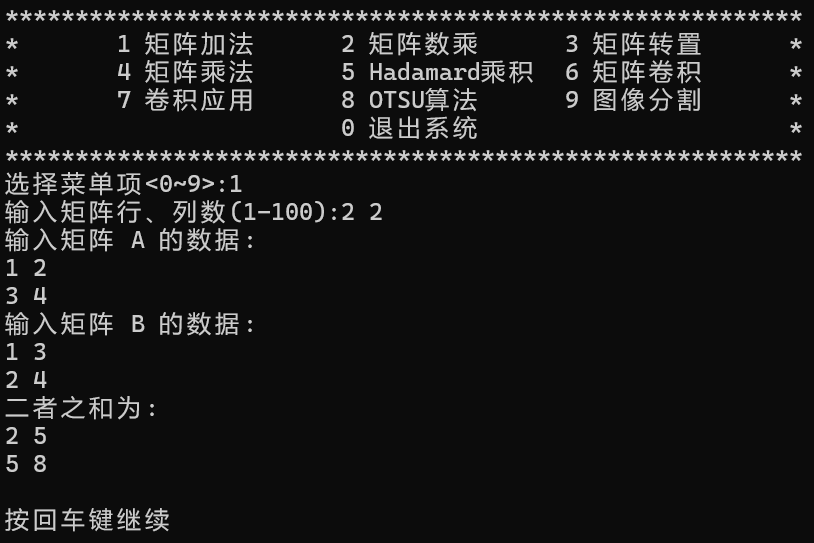
\includegraphics[width=.3\textwidth]{menu_and_1.jpg}
    \quad
    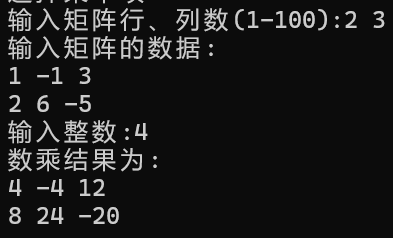
\includegraphics[width=.3\textwidth]{2.jpg}
    \quad
    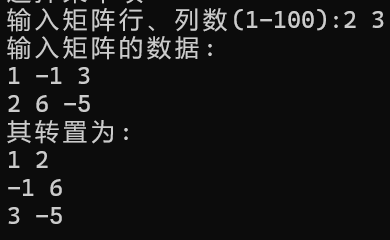
\includegraphics[width=.3\textwidth]{3.jpg}\\
    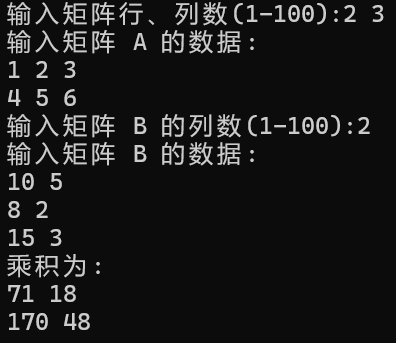
\includegraphics[width=.3\textwidth]{4.jpg}
    \quad
    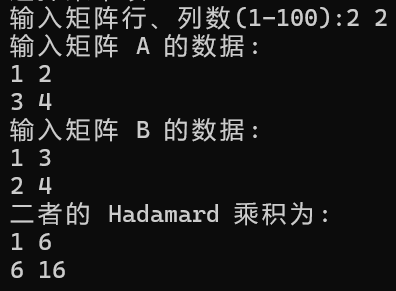
\includegraphics[width=.3\textwidth]{5.jpg}
    \quad
    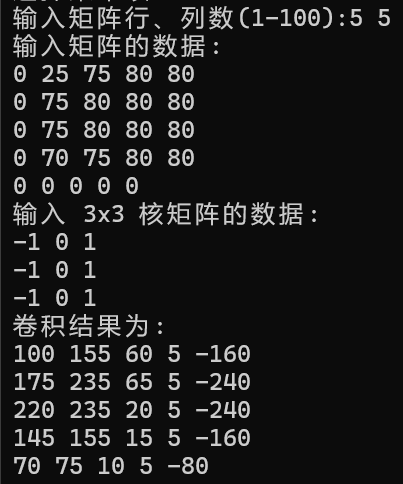
\includegraphics[width=.3\textwidth]{6.jpg}
    \caption{菜单及各功能(除图像处理)}
\end{figure}



\subsection{设计思路}

首先,加分项推荐使用一维数组,因此本程序所有矩阵均使用一维数组存储.其次,考虑到后续图像最大尺寸为 \verb|256*256| 且矩阵数据没有涉及小数(除了二值化将涉及 \verb|double|),故数组类型均为 \verb|int|.并且,对于非图像功能,不妨设置矩阵的最大尺寸为 \verb|MAXN = 100| 以节省栈 (本程序不使用动态 \verb|vector|)\footnote{缺陷就是,前面的计算功能不能设计浮点数计算和大矩阵计算.}.

从 \verb|main()| 出发,输入用户选择涉及一个 \verb|char| 类型变量 \verb|choice|,不妨设置为全局的.在 \verb|main()| 之前设置若干功能的对应函数.首先是参考模版的暂停函数 \verb|wait_for_enter()| 和菜单显示函数 \verb|menu()|.并且,考虑到输入矩阵行列、矩阵数据的操作在许多功能里都要涉及,故单独定义全局 \verb|int| 整型 \verb|raw,col|,并定义好行列输入函数 \verb|inputRC()| 和数据输入函数 \verb|inputMatrix()| 以备后续之需.其中注意,但凡用户输入非整型数据,直接以 \verb|exit(0)| 退出程序.输入行列时考虑取值范围.而由于只使用一维数组,输入矩阵数据可直接仅用 1 个循环搞定,遍历 \verb|raw*col|.

接着是各功能实现,直到图片设置之前,都仅是处理数组数据而没有涉及 \verb|opencv|.然而,由于各功能涉及的运算不同,循环内容是不同的.因此,我们并没有单独定义一个存储结果的数组、显示其数据的函数.实际上,直接在循环内容中写 \verb|cout| 即可.

具体实现过程很简单,故不赘述,已由末尾代码道尽.只提如下若干细节:
\begin{enumerate}
    \item 矩阵加法要求行列一致,故只需调用一次 \verb|inputRC()|,没必要再加代码去判断是否一致,强制用户输入正确(\verb|cin| 少了 \verb|iostream| 等着,多了可考虑清空缓冲区);
    \item 数乘输入那个数字时判断一下是否为整型;
    \item 转置功能实质是调换了双循环 \verb|i,j| 的嵌套顺序,但循环内容书写顺序仍为 \verb|i*col+j|;
    \item 对于矩阵乘法,同理地,调用一次 \verb|inputRC()| 之后只允许用户键入右乘矩阵的列数 \verb|int B_col|,其行数强制为左乘矩阵的列数,并注意范围和整型判断即可.矩阵 $A,B$ 的乘法为
    \eq{
        (AB)_{\mu\nu}=A_{\mu\lambda}B_{\lambda\nu},
    }
    其中使用 Einstein 求和约定.对 $\lambda$ 的求和在代码中表征为按 \verb|int z| 的循环,然后注意乘法格式为 \verb|matrixA[i * col + z] * matrixB[z * B_col + j]|;
    \item Hadamard 乘积无非是把矩阵加法的加号 \verb|+| 改为乘号 \verb|*|.
    \item 稍微难一点的是卷积过程,见 \ref{sec:conv} 节.
\end{enumerate}

此后功能均用到 \verb|opencv|.该库提供了一个实质为 \verb|uchar| 类型(一个像素点的灰度值遍历 $0\sim 255$)的二维数组类型 \verb|Mat|,且含 \verb|RGB| 三个通道的存储(故其实又带指针功能).定义 \verb|Mat image|,并
先用 \verb|imread()| 功能从具体图片(建议采用\textit{相对地址})中读取数据.以防万一加限制 \verb|IMREAD_GRAYSCALE|(\verb|demolena.jpg| 是含相等三通道数据的黑白图,用不用都行).在用 \verb|imshow()| 显示图片之前,不妨先用 \verb|namedWindow()| 设置成可调尺寸的窗口.本图尺寸 \verb|256*256|,故暂无需用 \verb|image.rows| 等去提取尺寸数据.

用 \verb|int matrix[256*256]| 存储 \verb|image|,但由于 \verb|Mat| 是二维的,我们还是得用双循环赋值.此处使用 \verb|image.ptr(i,j)[0]|,这里取其它通道也是一样的值因为这张图是黑白呈现的.

来到卷积应用.在此之前,用 \verb|int b| 的循环,遍历 $0\sim 5$,代表不同滤波器的核矩阵.而所有核矩阵数据存储在一个较大数组 \verb|int B[54]| 中,每次用 \verb|int kernel[9]| 截取即可,并顺便求出核矩阵之和 \verb|int kernel_sum| 以备平均化.后续卷积过程同理,只是注意加入如下细则:
\begin{enumerate}
    \item 若 \verb|kernel_sum| 不为零,则卷积结果除以它;
    \item 考虑到结果可能过黑(事实上核矩阵 $B_2,B_3,B_5$ 正是如此),可以在此处对这三种情况(用 \verb|if| 判断 \verb|b|),加偏移量 \verb|128|(所有像素)后呈现为灰色“浮雕”效果.当然,亦可不加,不加就注释掉;
    \item 噪点抹平,灰度超过 \verb|255| 的赋值 \verb|255|,为负数的赋 \verb|0|.
\end{enumerate}
之后用双循环把卷积结果的数组 \verb|result| 数据覆盖到 \verb|image.ptr(i, j)|.不用担心,原图的信息已由 \verb|matrix| 搞定,我们不会动它的.当然,实际上要写个 \verb|int n| 遍历三次的循环,将三个通道 \verb|image.ptr(i, j)[n]| 都赋为一致 \verb|result[i * 256 + j]|,才能出黑白图.
输出结果图像时,窗口的名称字符串用 \verb|b| 来排序即可.随后可等待若干秒自动关闭所有窗口,如 7 秒就是“\verb|if (waitKey(7000)) destroyAllWindows()|”.

\begin{figure}[ht]
    \centering
    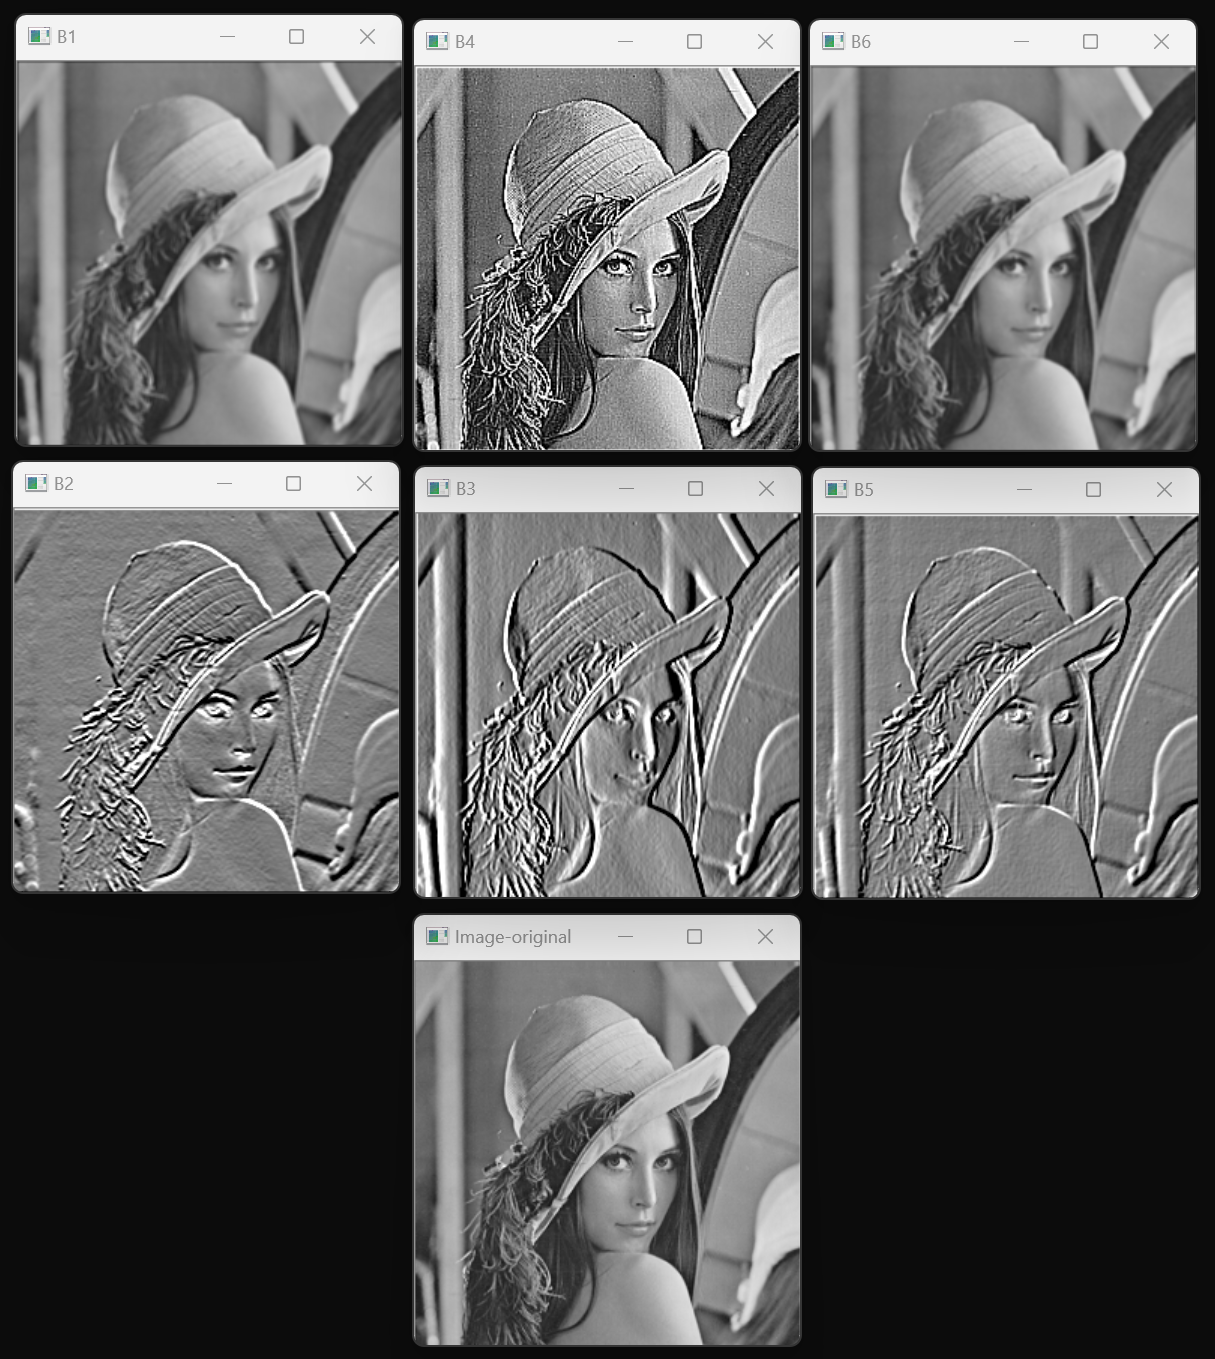
\includegraphics[width=.35\textwidth]{shift.jpg}
    \quad
    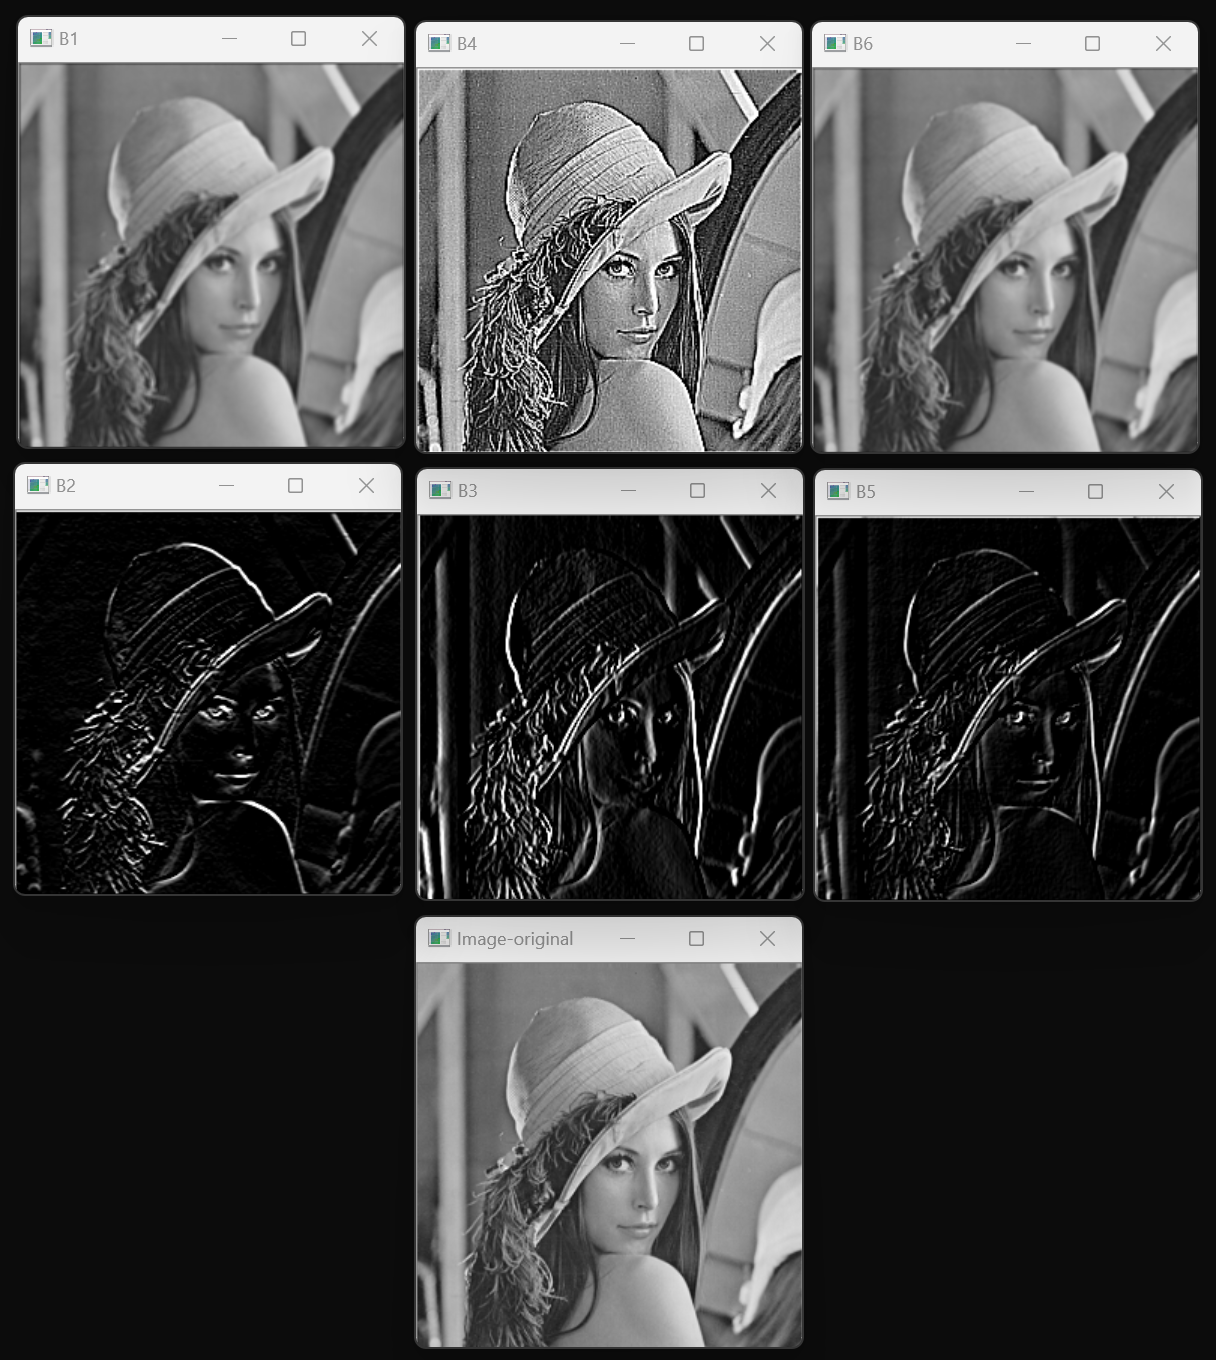
\includegraphics[width=.35\textwidth]{no_shift.jpg}
    \caption{加偏移量(左)和不加偏移量的效果}
\end{figure}

随后是 OTSU 二值处理.这一部分按 OTSU 的公式编写算法即可,也即根据图片计算出那个阈值 \verb|int threshold| 以供参考.凡大于该值的赋予白色,小于的赋予黑色.

\begin{figure}[ht]
    \centering
    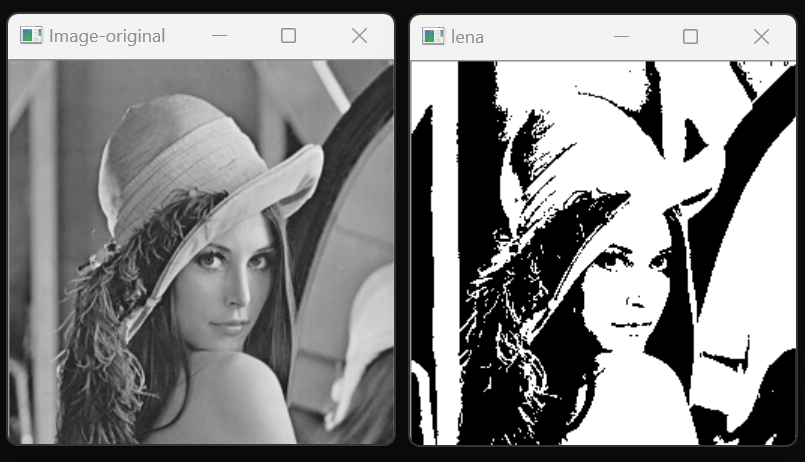
\includegraphics[width=.5\textwidth]{otsu.jpg}
    \caption{二值化}
\end{figure}

最后,抠图功能的原理差不多.利用 OTSU 算法粗略地思索,明显高于阈值的,标注为\textbf{前景},定位到原图,相应像素不变,剩下部分即\textbf{背景},像素取黑色.然而,OTSU 算法的优化极限(具体优化见 \ref{sec:OTSUseg} 节)仍有明显缺陷,故其实最好再采用新算法(结合边缘检测、区域生长、水平集方法等).本次作业为方便暂用 OTSU 算法的逻辑符优化.

\begin{figure}[ht]
    \centering
    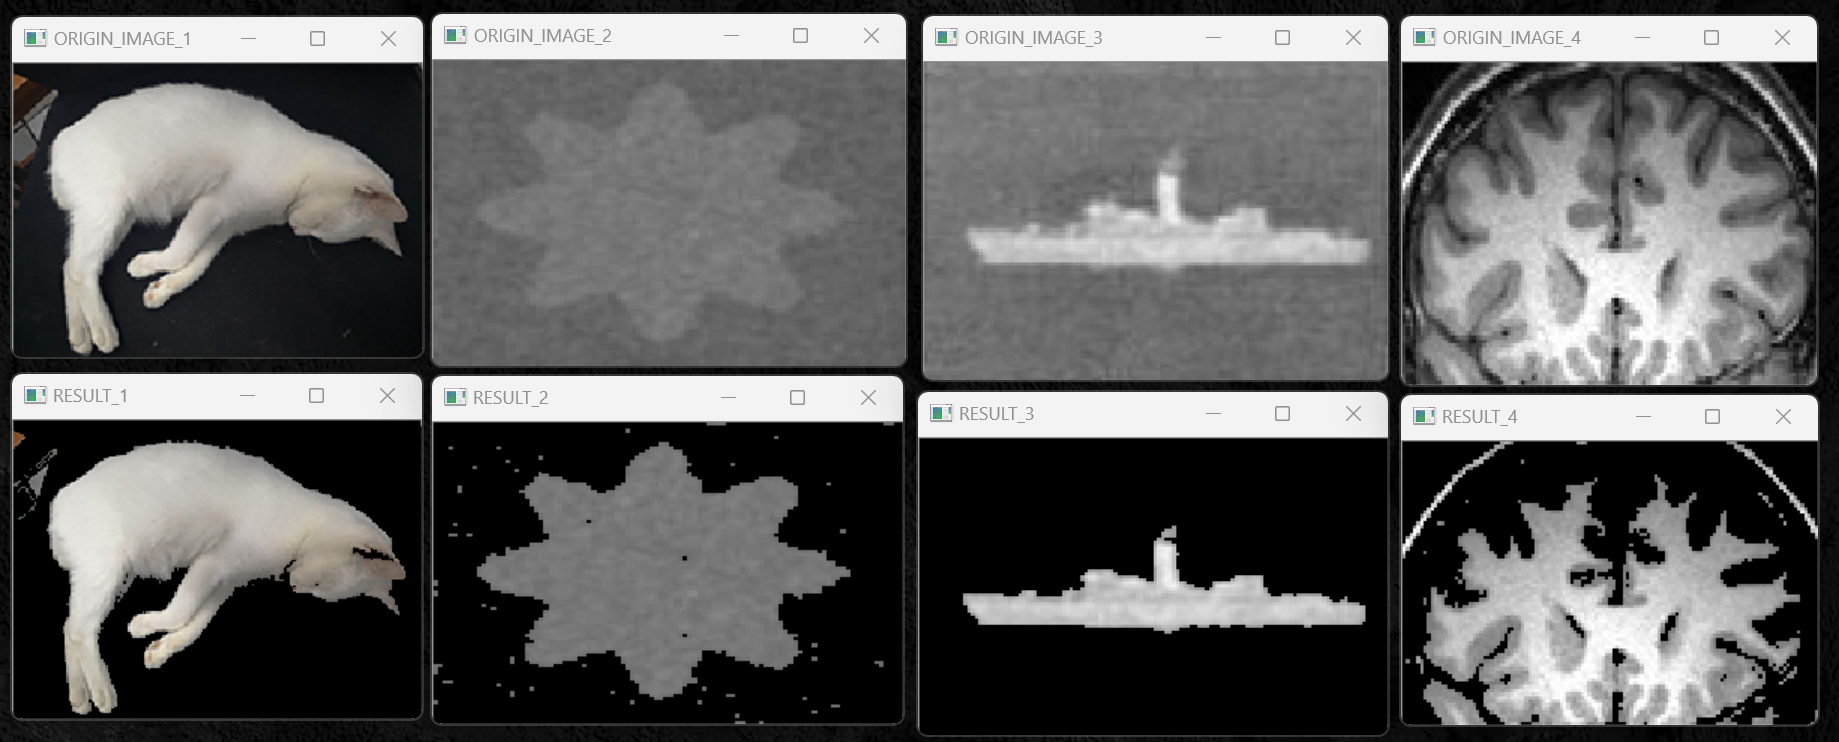
\includegraphics[width=.6\textwidth]{seg.jpg}
    \caption{图像分割}
\end{figure}



\newpage
\section{问题及解决方法}
\subsection{一维数组的使用}
注意定义矩阵时,二维写法 \verb|matrix[MAXN][MAXN]| 改成 \verb|matrix[MAXN*MAXN]|,而双循环内矩阵元写法从 \verb|matrix[i][j]| 改为 \verb|matrix[i*col + j]|,其中 \verb|col| 处不一定是列数,视 \verb|j| 的取值而定.基本上只涉及这种细节易错点而无大碍.

\subsection{卷积原理}\label{sec:conv}
由于有默认的卷积参数,故不必再单独设置那些变量,皆用数字直接手算进算法里,得到最简洁的:
\begin{lstlisting}[
    caption     =   {\bf conv()},
]
for (int x = 0; x < raw; ++x) {
    for (int y = 0; y < col; ++y) { // 遍历卷积核
        for (int i = -1; i <= 1; ++i) {
            for (int j = -1; j <= 1; ++j) {
                int nx = x + i;
                int ny = y + j;
                if (nx >= 0 && nx < raw && ny >= 0 && ny < col) { // 检查边界,处理边界外为0的情况
                    result[x * col + y] += matrix[nx * col + ny] * kernel[(i + 1) * 3 + (j + 1)];
                }
            }
        }
    }
}
\end{lstlisting}
其中注意先把 \verb|result| 全初始化为零.

\subsection{OpenCV 配置}
本次作业所提供的教程并不完全.首先,只考虑了学生设备的 CPU 为 x64 架构,未考虑 arm,如还算较为畅销的新版 Mac(即使非 MacOS,也存在 arm 版本 Windows 之可能).其次,教程声称“\textit{配置一次之后,所有新建项目都能应用此配置,不需要进行重复的配置操作}”,但实质上还要有一些教程未讲解的额外操作,此处不赘述.注意,对 arm 架构,debug 和编译设置都应保持相应状态.实在遇到重重难题的,\textit{可考虑淘宝或闲鱼服务}.
MacOS 下推荐 VScode + Cpp插件 + Copilot + OpenCV(arm) 的搭配,除非设备为老款 intel Mac.

如实在遇到缺少某个 \verb|dll| 文件或 \verb|exception| 内存地址的问题,自行 Google,Wiki 或丢给 ChatGPT.这种问题由于本人未直接处理 \verb|Mat|,实际上未遇到.

\subsection{栈溢出(stack overflow)}
考虑动态数组(\verb|vector| 也算一维的)或只设置足够小的 \verb|MAXN|.对于 \verb|int| 类型,推荐不超过 \verb|500|.若实在想进行浮点数的矩阵运算,对于 \verb|double| 类型,推荐不超过 \verb|200|.




\subsection{图像处理}
首先是要自己查阅有关 OpenCV 提供的各种功能函数的资料.\verb|ptr| 是比 \verb|at| 更快的(后者含边界判断等步骤),且也能更方便处理颜色通道(语法更简单).

\begin{figure}[ht]
    \centering
    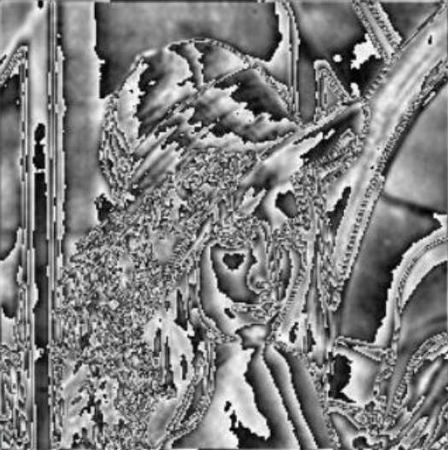
\includegraphics[width=.3\textwidth]{metal.png}
    \caption{$B_1$ 的“金属”样貌}
\end{figure}

避免使用 \verb|filter2D| 等自动处理卷积的函数,其本质是处理 \verb|uchar|.超过其范围会按 $0\sim 255$ 轮回,可能出现不断黑白突变的情况,尤其是忘记除以 \verb|kernel_sum| 时).
注意,除的时候一定要判断是否非零,否则可能会因为除法报错使结果非黑即白(或灰),如默认存储值 0 即黑色.
直接操作 \verb|Mat| 还可能带来若干问题.
\begin{figure}[ht]
    \centering
    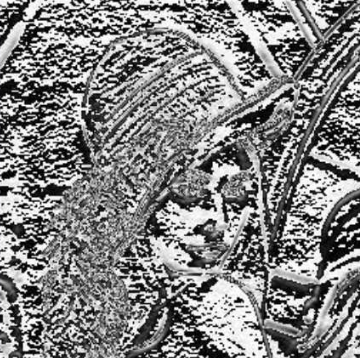
\includegraphics[width=.3\textwidth]{kernel2.png}
    \quad
    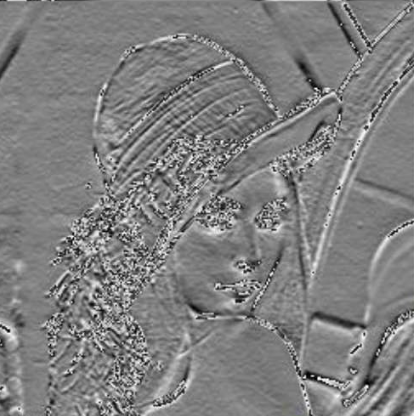
\includegraphics[width=.3\textwidth]{kernel2_no_if.png}
    \caption{$B_2$ 的“铜版画”样貌以及黑白噪点}
\end{figure}
如不加偏移量,在 $B_2$ 可能出现“铜版画”样貌.即使加上偏移量,也仍然有噪点.
包括 $B_4$ 也可能出现噪点.
\begin{figure}[ht]
    \centering
    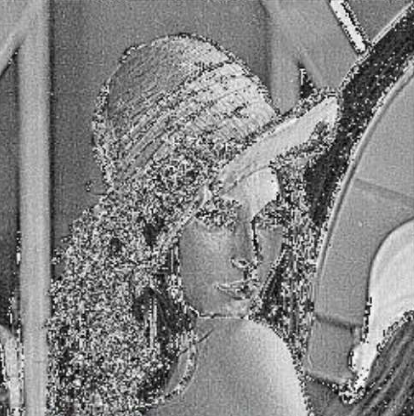
\includegraphics[width=.3\textwidth]{kernel4.png}
    \caption{$B_4$ 噪点}
\end{figure}
出现噪点就意味着要对越界值强制改为 \verb|0| 或 \verb|255|,即抹平操作.此外,使用 \verb|Mat| 或动态 \verb|vector| 还可能会遇到只绘制左 1/3 的情形.本人一开始就是用 \verb|int| 数组,故没有遇到此种情形.此处截图为他人所遇之.
\begin{figure}[ht]
    \centering
    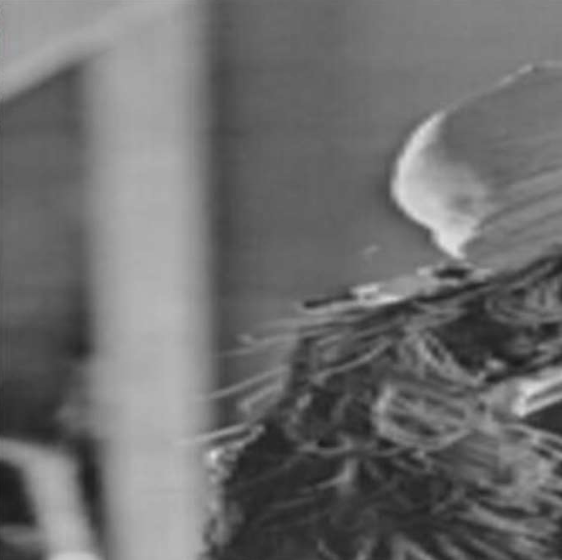
\includegraphics[width=.3\textwidth]{frac13.png}
    \caption{左 $1/3$ 不完整绘制}
\end{figure}

\textbf{一个至关重要的技巧}:如果不确定卷积结果、除以结果、越界结果是否正确,可以写双循环输出左上角 $15\times 15$ 的原图、结果数据进行判断和代码修改.若功能 6 保证正确,可用功能 6 进行计算以比较.对着错误的杂乱图像,反而不能直观看到哪里出现计算错误.

为避免 \verb|uchar| 的这些各种奇葩弊端,以及更多关于 \verb|opencv|、图像格式及色彩空间的知识(以免耽误时间错过作业提交期限),最好不要直接处理 \verb|Mat| 变量,而是改用 \verb|int| 存储数据.因此,基本上需要自己写卷积算法来处理数组了.反正功能 6 都得自己写,何不直接搬来?


窗口命名请务必用字符串加法和 \verb|int b| 的提取 \verb|to_string(b + 1)|,这里加一是为了对齐 $1\sim 6$.注意引号均用双引号.此外一定要跟一个 \verb|waitKey()|,否则图片会卡住,不能正常显示.非要用 \verb|waitKey(0)| 退出的话,注意请找到单击出现的图片窗口(时间太快就选代码中最后的,如 $B_6$),再按任意键,对桌面或 \verb|cmd| 窗口按都没用.

\subsection{OTSU 算法原理}
设灰度值阈值 $T$ 将各图像像素分为两类 $B,F$.记分别属于 $B,F$ 类的数量为 $w_B,w_F$,以 $w_\text{ts}=R\times C$ 代表图像总像素(ts指total size),则各自的区间概率为
\[
    p_B=\frac{w_B}{w_\text{ts}},\quad p_F=\frac{w_F}{w_\text{ts}}.
\]
其满足 $w_B+w_F=w_\text{ts}$ 或 $p_B+p_F=1$.设 $S_\text{ts}$ 是所有像素灰度值总和,类似地记 $S_B,S_F$,则 $S_\text{ts}=S_B+S_F$.
记总像素灰度均值为 $m_\text{ts}$,类似地记 $m_B,m_F$,则有
\[
    m_\text{ts}=\frac{S_\text{ts}}{w_\text{ts}}=\frac{w_B}{w_\text{ts}}\frac{S_B}{w_B}+\frac{w_F}{w_\text{ts}}\frac{S_F}{w_F}=p_B m_B+p_Fm_F.
\]
即 $m_\text{ts}$ 是 $m_B,m_F$ 的加权平均.
\textbf{类间方差}(intra-class variance)定义为
\eq{
    \sigma^2_b=p_B(m_B-m_\text{ts})^2+p_F(m_F-m_\text{ts})^2,
}
则可化简得
\eq{
    \sigma^2_b=p_Bp_F(m_B-m_F)^2,
}
目的是找到使其最大的 $T$.实际计算中从直方图出发,记位灰度值为 $i$ 的像素个数为 $H_i$,位于该值的概率为 $p_i={H_i}/{w_\text{ts}}$,则有
\eq{
    w_\text{ts}=\sum_{i=0}^{255} H_i,\quad p_B=\sum_{i=0}^{T}p_i,\quad S_\text{ts}=\sum_{i=0}^{255} i H_i,\quad m_B =   \frac{\sum_{i=0}^{T}iH_i}{\sum_{i=0}^{T} H_i}=\sum_{i=0}^{T}i\frac{p_i}{p_B}.
}
并且,考虑到只需要比较方差的大小,因此可以考虑重新定义
\eq{
    \mathtt{varBetween}=w_B w_F (m_B-m_F)^2,
}
即为代码中实际计算的“方差”,从而省去对概率 $p_i,p_B$ 等的计算.

\begin{lstlisting}[
    caption     =   {\bf OTSU()},
]
int threshold = 0; //灰度值阈值

int sumB = 0;
int wB = 0;
int wF = 0;
double mB;
double mF; //各自均值
double varMax = 0; //最大方差
double varBetween; //类间方差

int histogram[256]{};//灰度值直方图
for (int i = 0; i < image.rows; ++i) {
    for (int j = 0; j < image.cols; ++j) {
        histogram[image.ptr(i, j)[0]]++;
    }
}

int sum = 0;
for (int i = 1; i < 256; ++i) {
    sum += i * histogram[i]; //各像素灰度值总和
}

for (int i = 0; i < 256; ++i) {
    wB += histogram[i];
    if (wB == 0) continue; //为零导致方差为零,不是最大的
    wF = image.rows * image.cols - wB;
    if (wF == 0) break; //说明已经完成最大值查找
    sumB += i * histogram[i];
    mB = (double)sumB / wB;
    mF = ((double)sum - (double)sumB) / wF;
    varBetween = wB * wF * (mB - mF) * (mB - mF);
    if (varBetween > varMax) {
        varMax = varBetween;  //更新最大方差与阈值
        threshold = i;
    }
}
\end{lstlisting}

\subsection{OTSU 分割及其优化}\label{sec:OTSUseg}
直接按灰度图得到唯一阈值固然是可以的,然而为更好处理边界像素点,可以综合考虑原图的三通道阈值,尤其对猫图 \verb|snowball.jpg|.一般按逻辑运算符或加权融合确定最终的前景像素:
\begin{itemize}
    \item 逻辑与,只有当一个像素在所有三个通道的二值化结果中均为前景时,它才被认定为最终的前景.这通常会得到较为严格、边界更清晰的前景;
    \item 逻辑或,如果一个像素在任一通道的二值化结果中为前景,它就被认定为前景.这会得到更全面的前景覆盖,但可能包括更多的噪声;
    \item 加权融合,可以根据场景的具体需求对不同通道的结果进行加权融合,例如,如果某一颜色通道对前景的贡献更大(比如偏绿的丛林、泛黄的老照片),则可以给予更高的权重.
\end{itemize}
结果显示,逻辑或(注意源代码中是确定背景像素,因此逻辑符号反过来写成 \verb|and|)的效果好于逻辑与,且加权融合的权重设置实质上意义不大,故可以说 OTSU 算法的优化极限是逻辑或了.


\newpage
\section{心得体会}
\subsection{所思所感及吐槽}
配置环境和 debug 果然是最费时间的.

现在已步入 AI 时代,借助 AI 编写经典算法可以保证简洁代码量和低时间复杂度.故在学习和工作中均建议配合使用,多将人类的头脑花在非机械性的创造、思考工作上.

当然,亦不可轻信 AI,务必善用搜索引擎和百科文库查找具体资料.

切勿放纵而浮躁\footnote{本文档采用 \LaTeX 编写,考验笔者之耐心.}.peace$\sim$



\subsection{对图像卷积操作的理解}

主要是谈那六个滤波器的直观含义.卷积核之和与 1 
的相对大小表征处理后的图像亮度,除以该和可保持大概一致的亮度,除非该和为零时可能需要加偏移量.可看出六个核矩阵的对应情况如下.
\begin{enumerate}
    \item 模糊,将本像素点与周遭进行直接平均,达到平滑化效果:
    \[\left[\begin{array}{ccc}1 & 1 & 1 \\ 1 & 1 & 1 \\ 1 & 1 & 1\end{array}\right];\]
    \item 浮雕,将不同侧像素点之间的差别放大,一边乘正数而变亮,一边乘负数而便暗,模拟出侧面光照的效果.此处是上下差别:
    \[\left[\begin{array}{ccc}-1 & -2 & -1 \\ 0 & 0 & 0 \\ 1 & 2 & 1\end{array}\right];\]
    \item 浮雕,左右差别:
    \[\left[\begin{array}{ccc}-1 & 0 & 1 \\ -2 & 0 & 2 \\ -1 & 0 & 1\end{array}\right];\]
    \item 锐化,在用本像素点与周围像素点作差再加权来放大这种差别(中心元素为很大的 $9$,周围取 $-1$),使各像素点特点在卷积后突出:
    \[\left[\begin{array}{ccc}-1 & -1 & -1 \\ -1 & 9 & -1 \\ -1 & -1 & -1\end{array}\right];\]
    \item 浮雕,左上与右下的差别:
    \[\left[\begin{array}{ccc}-1 & -1 & 0 \\ -1 & 0 & 1 \\ 0 & 1 & 1\end{array}\right];\]
    \item Gauss 模糊,将本像素点与周遭进行按二维 Gauss 分布的有层次的平均:
    \[\left[\begin{array}{ccc}1 & 2 & 1 \\ 2 & 4 & 2 \\ 1 & 2 & 1\end{array}\right].\]
\end{enumerate}






\newpage
\section{源代码}
\begin{lstlisting}[
    caption     =   {\bf main.cpp},
    label       =   {code}
]
#include <conio.h> //可能与 cout 冲突
#include <iostream>
#include <opencv2/opencv.hpp>
using namespace cv;
using namespace std;

const int MAXN = 100; //最大阶数
char choice;

int raw, col;

void wait_for_enter() {
    cout << "\n按回车键继续";
    while (_getch() != '\r');
    cout << "\n\n";
}
void inputRC() {
    cout << "输入矩阵行、列数(1-" << MAXN << "):";
    while (1) {
        cin >> raw >> col;
        if (cin.fail()) {
            cout << "输入错误,非整数!退出程序!";
            exit(0);
        }
        else if (raw >= 1 and raw <= MAXN
            and col >= 1 and col <= MAXN) {
            break;
        }
        cout << "超出范围,请重新输入:";
    }
}
void inputMatrix(int matrix[MAXN * MAXN]) {
    for (int i = 0; i < raw * col; ++i) {
        cin >> matrix[i];
        if (cin.fail()) {
            cout << "输入错误,非整数!退出程序!";
            exit(0);
        }
    }
}
void menu() {
    for (int i = 1; i <= 57; ++i) cout << "*";
    cout << "\n*       1 矩阵加法      2 矩阵数乘      3 矩阵转置      *";
    cout << "\n*       4 矩阵乘法      5 Hadamard乘积  6 矩阵卷积      *";
    cout << "\n*       7 卷积应用      8 OTSU算法      9 图像分割      *";
    cout << "\n*                       0 退出系统                      *\n";
    for (int i = 1; i <= 57; ++i) cout << "*";
    cout << "\n选择菜单项<0~9>:";        // 按要求输入菜单选择项choice
    cin >> choice;
}
void matriplus() {
    inputRC();

    cout << "输入矩阵 A 的数据:\n";
    int matrixA[MAXN * MAXN];
    inputMatrix(matrixA);

    cout << "输入矩阵 B 的数据:\n";
    int matrixB[MAXN * MAXN];
    inputMatrix(matrixB);

    cout << "二者之和为:\n";
    for (int i = 0; i < raw; ++i) {
        for (int j = 0; j < col; ++j) {
            cout << matrixA[i * col + j] + matrixB[i * col + j] << ' ';
        }
        cout << endl;
    }
    wait_for_enter();
}
void nummulti() {
    inputRC();

    cout << "输入矩阵的数据:\n";
    int matrix[MAXN * MAXN];
    inputMatrix(matrix);

    cout << "输入整数:";
    int k;
    cin >> k;
    if (cin.fail()) {
        cout << "输入错误,非整数!退出程序!";
        exit(0);
    }

    cout << "数乘结果为:\n";
    for (int i = 0; i < raw; ++i) {
        for (int j = 0; j < col; ++j) {
            cout << k * matrix[i * col + j] << ' ';
        }
        cout << endl;
    }
    wait_for_enter();
}
void matritrans() {
    inputRC();

    cout << "输入矩阵的数据:\n";
    int matrix[MAXN * MAXN];
    inputMatrix(matrix);

    cout << "其转置为:\n";
    for (int j = 0; j < col; ++j) {
        for (int i = 0; i < raw; ++i) {
            cout << matrix[i * col + j] << ' ';
        }
        cout << endl;
    }
    wait_for_enter();
}
void matrimulti() {
    inputRC();

    cout << "输入矩阵 A 的数据:\n";
    int matrixA[MAXN * MAXN];
    inputMatrix(matrixA);

    cout << "输入矩阵 B 的列数(1-" << MAXN << "):";
    int B_col;
    while (1) {
        cin >> B_col;
        if (cin.fail()) {
            cout << "输入错误,非整数!退出程序!";
            exit(0);
        }
        else if (B_col >= 1 and B_col <= MAXN) {
            break;
        }
        cout << "超出范围,请重新输入:";
    }

    cout << "输入矩阵 B 的数据:\n";
    int matrixB[MAXN * MAXN];
    for (int i = 0; i < col * B_col; ++i) {
        cin >> matrixB[i];
        if (cin.fail()) {
            cout << "输入错误,非整数!退出程序!";
            exit(0);
        }
    }

    int sum = 0;
    cout << "乘积为:\n";
    for (int i = 0; i < raw; ++i) {
        for (int j = 0; j < B_col; ++j) {
            for (int z = 0; z < col; ++z) {
                sum += matrixA[i * col + z] * matrixB[z * B_col + j];
            }
            cout << sum << ' ';
            sum = 0;
        }
        cout << endl;
    }
    wait_for_enter();
}
void hadamulti() {
    inputRC();

    cout << "输入矩阵 A 的数据:\n";
    int matrixA[MAXN * MAXN];
    inputMatrix(matrixA);

    cout << "输入矩阵 B 的数据:\n";
    int matrixB[MAXN * MAXN];
    inputMatrix(matrixB);

    cout << "二者的 Hadamard 乘积为:\n";
    for (int i = 0; i < raw; ++i) {
        for (int j = 0; j < col; ++j) {
            cout << matrixA[i * col + j] * matrixB[i * col + j] << ' ';
        }
        cout << endl;
    }
    wait_for_enter();
}
void conv() {
    inputRC();

    cout << "输入矩阵的数据:\n";
    int matrix[MAXN * MAXN];
    inputMatrix(matrix);

    cout << "输入 3x3 核矩阵的数据:\n";
    int kernel[9];
    for (int i = 0; i < 9; ++i) {
        cin >> kernel[i];
    }

    int result[MAXN * MAXN]{};
    for (int x = 0; x < raw; ++x) {
        for (int y = 0; y < col; ++y) { // 遍历卷积核
            for (int i = -1; i <= 1; ++i) {
                for (int j = -1; j <= 1; ++j) {
                    int nx = x + i;
                    int ny = y + j;
                    if (nx >= 0 && nx < raw && ny >= 0 && ny < col) { // 检查边界,处理边界外为0的情况
                        result[x * col + y] += matrix[nx * col + ny] * kernel[(i + 1) * 3 + (j + 1)];
                    }
                }
            }
        }
    }

    cout << "卷积结果为:\n";
    for (int i = 0; i < raw; ++i) {
        for (int j = 0; j < col; ++j) {
            cout << result[i * col + j] << " ";
        }
        cout << endl;
    }
    wait_for_enter();
}
void demo() {
    int B[54]{ 1, 1, 1, 1, 1, 1, 1, 1, 1,
             -1, -2, -1, 0, 0, 0, 1, 2, 1,
             -1, 0, 1, -2, 0, 2, -1, 0, 1,
             -1, -1, -1, -1, 9, -1, -1, -1, -1,
             -1, -1, 0, -1, 0, 1, 0, 1, 1,
             1, 2, 1, 2, 4, 2, 1, 2, 1 },
        kernel[9];

    Mat image = imread(".//image//demolena.jpg"); // 图像的灰度值存放在格式为Mat的变量image中
    namedWindow("Image-original", WINDOW_NORMAL);
    imshow("Image-original", image);

    int matrix[256 * 256];
    for (int i = 0; i < 256; ++i) {
        for (int j = 0; j < 256; ++j) {
            matrix[i * 256 + j] = image.ptr(i, j)[0];
        }
    }

    for (int b = 0; b < 6; ++b) {
        int kernel_sum = 0; //求卷积核的和
        for (int k = 0; k < 9; ++k) {
            kernel[k] = B[b * 9 + k];
            kernel_sum += kernel[k];
        }

        int result[256 * 256]{};
        for (int x = 0; x < 256; ++x) {
            for (int y = 0; y < 256; ++y) {
                for (int i = -1; i <= 1; ++i) {
                    for (int j = -1; j <= 1; ++j) {
                        int nx = x + i;
                        int ny = y + j;
                        if (nx >= 0 && nx < 256 && ny >= 0 && ny < 256) {
                            result[x * 256 + y] += matrix[nx * 256 + ny] * kernel[(i + 1) * 3 + (j + 1)];
                        }
                    }
                }
                if (kernel_sum != 0) {
                    result[x * 256 + y] /= kernel_sum;
                }
                if (b == 1 or b == 2 or b == 4) {
                    result[x * 256 + y] += 128;    // 对亮度过低的可以加偏移量
                }
                if (result[x * 256 + y] > 255) {
                    result[x * 256 + y] = 255;
                }
                else if (result[x * 256 + y] < 0) {
                    result[x * 256 + y] = 0;
                }
            }
        }

        for (int i = 0; i < 256; ++i) {
            for (int j = 0; j < 256; ++j) {
                image.ptr(i, j)[0] = image.ptr(i, j)[1] = image.ptr(i, j)[2] = result[i * 256 + j];
            }
        }
        string name = "B" + to_string(b + 1);
        namedWindow(name, WINDOW_NORMAL);
        imshow(name, image);
    }
    if (waitKey(30000)) destroyAllWindows();
}
void OTSU() {
    Mat image = imread(".//image//demolena.jpg");
    namedWindow("Image-original", WINDOW_NORMAL);
    imshow("Image-original", image);     

    int threshold = 0; //灰度值阈值

    int sumB = 0;
    int wB = 0;
    int wF = 0;
    double mB;
    double mF; //各自均值
    double varMax = 0; //最大方差
    double varBetween; //类间方差

    int histogram[256]{};     //灰度值直方图
    for (int i = 0; i < 256; ++i) {
        for (int j = 0; j < 256; ++j) {
            histogram[image.ptr(i, j)[0]]++;
        }
    }

    int sum = 0;
    for (int i = 1; i < 256; ++i) {
        sum += i * histogram[i]; //各像素灰度值总和
    }

    for (int i = 0; i < 256; ++i) {
        wB += histogram[i];
        if (wB == 0) continue; //为零导致方差为零,不是最大的
        wF = 256 * 256 - wB;
        if (wF == 0) break; //说明已经完成最大值查找
        sumB += i * histogram[i];
        mB = (double)sumB / wB;
        mF = ((double)sum - (double)sumB) / wF;
        varBetween = wB * wF * (mB - mF) * (mB - mF);
        if (varBetween > varMax) {
            varMax = varBetween;  //更新最大方差与阈值
            threshold = i;
        }
    }
    //二值化
    for (int i = 0; i < 256; ++i) { 
        for (int j = 0; j < 256; ++j) {
            image.ptr(i, j)[0] = image.ptr(i, j)[0] > threshold ? 255 : 0;
            image.ptr(i, j)[1] = image.ptr(i, j)[1] > threshold ? 255 : 0;
            image.ptr(i, j)[2] = image.ptr(i, j)[2] > threshold ? 255 : 0;
        }
    }

    namedWindow("lena", WINDOW_NORMAL);
    imshow("lena", image);
    if (waitKey(30000)) destroyAllWindows();
}
void seg() {
    string path[4] = { "snowball","polyhedrosis","ship","brain" };
    for (int imageN = 0; imageN < 4; ++imageN) {
        Mat image = imread(".//image//" + path[imageN] + ".jpg"); // 原图
        string name = "ORIGIN_IMAGE_" + to_string(imageN + 1);
        namedWindow(name, WINDOW_NORMAL);
        imshow(name, image);

        int threshold[3]{};
        for (int n = 0; n < 3; ++n) {
            int sumB = 0;
            int wB = 0;
            int wF = 0;
            double mB;
            double mF;
            double varMax = 0;
            double varBetween;
            int histogram[256]{};
            for (int i = 0; i < image.rows; ++i) {
                for (int j = 0; j < image.cols; ++j) {
                    histogram[image.ptr(i, j)[n]]++;
                }
            }
            int sum = 0;
            for (int i = 1; i < 256; ++i) {
                sum += i * histogram[i];
            }
            for (int i = 0; i < 256; ++i) {
                wB += histogram[i];
                if (wB == 0) continue;
                wF = image.rows * image.cols - wB;
                if (wF == 0) break;
                sumB += i * histogram[i];
                mB = (double)sumB / wB;
                mF = ((double)sum - (double)sumB) / wF;
                varBetween = wB * wF * (mB - mF) * (mB - mF);
                if (varBetween > varMax) {
                    varMax = varBetween;
                    threshold[n] = i;
                }
            }
        }
        //抠图,按逻辑运算符
        for (int i = 0; i < image.rows; ++i) {
            for (int j = 0; j < image.cols; ++j) {
                if (image.ptr(i, j)[0] < threshold[0] and image.ptr(i, j)[1] < threshold[1] and image.ptr(i, j)[2] < threshold[2])
                    image.ptr(i, j)[0] = image.ptr(i, j)[1] = image.ptr(i, j)[2] = 0;
            }
        }

        string result_name = "RESULT_" + to_string(imageN + 1);
        namedWindow(result_name, WINDOW_NORMAL);
        imshow(result_name, image);
    }
    if (waitKey(30000)) destroyAllWindows();
}

int main() {
    wait_for_enter();
    while (true) { // 注意该循环退出的条件
        system("cls"); // 清屏
        menu(); // 菜单
        if (choice == '0') { // 选择退出
            cout << "\n 确定退出吗? (y/n):";
            cin >> choice;
            if (choice == 'y' || choice == 'Y')
                break;
            else
                continue;
        }
        switch (choice) {
        case '1':
            matriplus();
            break;
        case '2':
            nummulti();
            break;
        case '3':
            matritrans();
            break;
        case '4':
            matrimulti();
            break;
        case '5':
            hadamulti();
            break;
        case '6':
            conv();
            break;
        case '7':
            demo();
            break;
        case '8':
            OTSU();
            break;
        case '9':
            seg();
            break;
        default:
            cout << "\n 输入错误,请重新输入\n";
            wait_for_enter();
        }
    }
    return 0;
}
\end{lstlisting}

\end{document}